
\documentclass{article}

% Recommended, but optional, packages for figures and better typesetting:
\usepackage{microtype}
\usepackage{algorithm}
\usepackage{algorithmic}
\usepackage{graphicx}
\usepackage{subfig}
\usepackage{natbib}
\usepackage{booktabs} % for professional tables
\usepackage{amsmath,amssymb}
\DeclareMathOperator{\E}{\mathbb{E}}

% hyperref makes hyperlinks in the resulting PDF.
% If your build breaks (sometimes temporarily if a hyperlink spans a page)
% please comment out the following usepackage line and replace
% \usepackage{icml2019} with \usepackage[nohyperref]{icml2019} above.
\usepackage{hyperref}

% Attempt to make hyperref and algorithmic work together better:
\newcommand{\theHalgorithm}{\arabic{algorithm}}

% Use the following line for the initial blind version submitted for review:
\usepackage[accepted]{icml2018}

% The \icmltitle you define below is probably too long as a header.
% Therefore, a short form for the running title is supplied here:
\icmltitlerunning{Music Neural Style Transfer}

\begin{document}

\twocolumn[
\icmltitle{Music Neural Style Transfer: \\ Transfering Style between Sparse Formats}

% It is OKAY to include author information, even for blind
% submissions: the style file will automatically remove it for you
% unless you've provided the [accepted] option to the icml2019
% package.

% List of affiliations: The first argument should be a (short)
% identifier you will use later to specify author affiliations
% Academic affiliations should list Department, University, City, Region, Country
% Industry affiliations should list Company, City, Region, Country

% You can specify symbols, otherwise they are numbered in order.
% Ideally, you should not use this facility. Affiliations will be numbered
% in order of appearance and this is the preferred way.
% \icmlsetsymbol{equal}{*}

\begin{icmlauthorlist}
\icmlauthor{Zhachory Volker}{}
\icmlauthor{Vladislava Paskova}{}
\end{icmlauthorlist}

% You may provide any keywords that you
% find helpful for describing your paper; these are used to populate
% the "keywords" metadata in the PDF but will not be shown in the document
\icmlkeywords{Machine Learning, ICML}

\vskip 0.3in
]

\begin{abstract}
Data generation is a hot topic nowadays. The use of GAN's, Variational Autoencoders, and Restricted Boltzman Machines are all examples of methods that can generate data. One method, which will focus on, is called Neural Style Tranfser. It takes the style of one image and places it into a content image. This method works very well, but is limited to dense data formats. We propose a method to utilize VAE's embedding power to shrink the size of sparse data formats to push through a Neural Style Transfer model. That way, for example, we could take the style from one piece of music and impose it on another. We will conduct experiments to prove that using the VAE model to preprocess music will create better and more realistic combination of two songs then without it. 
\end{abstract}

\section{Introduction}
\label{introduction}

Transfering style from one object to another is a complicated task, because what does it mean to impose style from an object onto another. In what ways do we describe that content is preserved by the style has changed. One solution for images is to use a Neural Style Transfer (NST) model. (Gatys et al., 2016) The NST model uses a pretrained network to grab it's understanding of both a content image and a style image and merge them together to create a stylized image. This model works well on images because images have dense data representations and there are have been a lot of research to improve image recognition and understanding, allowing for many robust pretrained networks to be available. 

Could this be done with other data types, such as music? The main problem with music data is that it is sparse. Music can be classified, at one step, by any number of 128 different keys being played at one time, with a variable amounts of force, timbre, length of note, and instrument. Along with that, music is temporal. The vector representation can be multiplied thousands of times, depending on how you extract the notes from music. However, whenever you listen to music, you can clearly identify different notes, instruments, beats, and other things in the music. This signifies that music's input space is on the scale millions while what could be played at one time is more down to the scale of tens.

Along with the sheer sparsity, music has a temporal structure. The main models that are used for temporal structures are LSTMs.(Hochreiter et al., 1997) Their long term structure suffers from well-document problems of "vanishing gradients" and "exploding gradients".(Sherstinsky, 2018)  These difficulties become pronounced when the dependencies in the target subsequence span a large number of samples, requiring the window of the unrolled RNN model to be commensurately wide in order to capture these long-range dependencies.

Both music's sparsity and its temporal structure defines the problems we must overcome if we would want to have style transfer for music.

We propose two improvements to handle these problems. One, will preprocess the music, which is coming in as MIDI data, with a Variational Autoencoder to get a lower dimensional representation of our input to feed into the Neural Style Transfer model to handle the sparsity. And two, we will utilize a custom 1D convolutional network to use as a backbone model for our NST model to handle music's temporal nature. We will prove our assumption that the VAE will represent music in a robust way so that, when passed through the NST, the data output will still represent the data distribution of the latent variables. This way we can decode it and get a stylized piece of music out.

\section{Background}
\label{background}

\subsection{Neural Style Transfer}

Gatys et al. first studied the power of CNNs to transform images from one style to another. The idea behind this increasingly popular method is as such: you have two types of images, a content and a style image, and you are trying to transfer the style from one image to the other. To do so we use two types of losses, often referred to as content and style loss. To capture global statistics and spatial arrangements we utilize a Gram matrix that is just the inner product between the the feature map of each images within a certain layer. (Jing et al., 2018) The content loss, denoted by Lc, is the squared Euclidean distance between the feature map of the content image and that of the style image in every layer of the pretrained network. We utilize a similar approach in our proposed neural music transfer methodology. 

\begin{equation} 
\begin{split}
	L_s & = \sum_{l \in {l_s}} || G(F^l(I_s)') - G(F^l(I))'||^2 \\
	L_c & = \sum_{l \in {l_c}} || F^l(I_c)') -  F^l(I)'||^2 \\
	L & = L_s + L_c \\
\end{split} 
\end{equation}

Equation 1: The style loss, the content loss , and the total loss are denoted by $L_s$, $L_c$, and $L$, respectively. ${l_s}$ and ${l_c}$ represent the model’s set of layers. $G$ is the gram matrix function. 

One of the most common networks used for neural style transfer in images is the VGG-19. Deep convolutional networks trained on classification tasks are used for style transfer because they have the style and content information encoded in their layers. (Jing et al., 2018)

\medskip

\subsection{MusicVae}

Music encoding has been a challenge within the machine learning community, because of its sparsity. To address this issue the Magenta team at Google has created a neural architecture for encoding music sequences. (Roberts et al, 2018)  Their model, Hierarchical Latent Vector Model, is a novel structure to encode long term structured sequences, such as music.(Roberts et al, 2018) They used a bidirectional LSTM layer structure to encode a long sequence of music into latent variables.(Schuster et al., 1997)  Once they sample from the encoded latent variables, they then use a 2-layer tree like decoder to parse through the encoding to generate music.

A VAE is a basic Autoencoder, but the latent codes are trained and sampled from a gaussian distribution.(Hinton et al., 2006) Because we are training a Variational Autoencoder, we want to minimize both the reconstruction error and the distribution divergence between our latent codes and a standard normal gaussian distributions.(Kingma et al., 2014) This can be achieved by maximizing the evidence lower bound (ELBO) which consists of maximizing the log likelihood of the reconstruction and minimizing the KL divergence.

\begin{equation} 
\begin{split}
	\E [ log p_\theta(x|z) ] - \beta KL(q_\lambda(z|x) || p(z))
\end{split} 
\end{equation}

Equation 2: ELBO denoted by E. Theta represents the model parameters, x is the input, z is the latent variables, and KL stands for KL divergence.

Setting $\beta < 1$ encourages the model to prioritize reconstruction quality over learning a compact representation (Higgins et al., 2017).

\textbf{Bidirectional Encoder} For the encoder $q_\lambda(z | x)$, they used a two-layer bidirectional LSTM network to produce latent codes from the last LSTM cell with these equations

\begin{equation} 
\begin{split}
	\mu & = W_{h_\mu}h_T + b_\mu \\
	\sigma & = log(exp(W_{h\sigma}h_T + b_\sigma) + 1) \\
\end{split} 
\end{equation}

Equation 3: The above equations represent the mean and standard deviation of the bidirectional encoder. Where the $W$s and $b$s are weight matrices and bias vectors, respectively. 

\textbf{Hierarchical Decoder} The hierarchical architecture of this decoder helps mitigate the vanishing influence of the latent state at the output sequence is being generated. Assume that the input sequence (and target output sequence) $x$ can be segmented into U non overlapping subsequences $y_u$ with endpoints $i_u$ so that

\begin{equation} 
\begin{split}
y_u & = { x_{i_u} , x_{i_u+1}, x_{i_u+2}, . . . , x_{i_{u+1}-1 } } \\
x & = {y_1, y_2, . . . , y_U } \\
\end{split} 
\end{equation} Equation 4.

where we define the special case of $i_U+1 = T$. Then, the latent vector z is passed through a fully-connected layer followed by a tanh activation to get the initial state of a “conductor” RNN. The conductor RNN produces $U$ embedding vectors $c = {c_1, c_2, . . . , c_U }$, one for each subsequence. The last unidirectional layer's cells take each subsequence individually to construct their portion of the reconstruction. 

We use this architecture to help encode music into a lower dimensional representation so that we may have a dense format to push into our Neural Style Transfer model. 


\section{Related Work}
\label{related}

Magenta's MusicVAE model could be manipulated to perform style transfer.(Roberts et al., 2018) The broad goal of an autoencoder is to learn a compact representation of the data. If we could coerce that representation to be put onto a latent space, we could utilize latent space manipulations to get a combination of two different pieces of music. For example, given two pieces of music latent representation, we could interpolate a path between their points in the latent space. We can pull points off that path and decode them to get a logical combination between both pieces. This can be perceived as putting style of piece onto another. 

However, what does style imply here? That is determined by the latent space and the path that is traverse. It is safe to assume that the traversal will be smooth and expected, since we are modeling some latent space. Unfortunately, this doesn't predict the optimal position in the path that optimizes that we keep the content of music 1 while imposing the style of music 2. We are essentially at the mercy of the latent space.

Another related project is the Music CycleGAN.(Brunner et al., 2018) A CycleGAN is a Generative Adversarial Network (GAN) that uses two networks and two discriminators.(Zhu et al., 2017) One generator brings in an image from class X and outputs an image from class Y and vice versa for the other generator. One discriminator is built to identify one class while the other is built for another. The objective for the generator is to fool the discriminator while the discriminator is trying to see which inputs are real or not. 

\begin{equation} 
\begin{split}
L_{adv}(G, D_y, X) & = \frac{1}{m} \sum_{i=1}^{m} (1 - D_y(G(x_i)))^2 \\
L_{adv}(F, D_y, X) & = \frac{1}{m} \sum_{i=1}^{m} (1 - D_x(F(y_i)))^2 \\
\end{split} 
\end{equation}

The cycle comes in when we first generate an image from $X$ to $Y$, then feed the generated $Y$ to the other generator to get a "reconstructed" $X$. The cycle loss is loss of information from between $X$ and the "reconstructed" $X$. The same can be done with samples from the $Y$ class. 

\begin{equation} 
\begin{split}
L_{cyc}(G, F, X, Y) & =  \frac{1}{m} \sum_{i=1}^{m} \left[ F(G(x_i)) - x_i \right] + \left[ G(F(y_i)) - y_i \right] \\
L & = L_{adv} + \lambda L_{cyc} \\
\end{split} 
\end{equation}

We can see how this can be augmented for music data. The generators could be either 1D convolution networks or recurrent neural networks to generate from one style of music to another. However, the user is limited to only going between style $X$ to style $Y$. Our method gives the user freedom to use any music they wish to represent their content and style. 


\section{Approach}
\label{approach}

In our experiments we aim to create a flexible infrastructure that can allows researchers to transfer music style. To address the issue of the sparse representation of music notes we propose an encoding and decoding step prior and after style. We hypothesize that this will densify the input and thus allow for a smoother style transfer. Furthermore, we plan to encode the data using a music VAE similar to Magenta. However, Magenta's input structure included monotonic sequencing that dropped chord structures and their library was very inflexible. Therefore, we created our own model which mimics Magenta's model architecture.

In addition, we propose the use of a different classifier than the VGG, most commonly used in image style transfer, as it is constructed to work on a three channeled data and music files have a temporal structure. We train our own convolutional classifier that predicts composers because we believe that the model will retain information about style and content given that each composer has a different style of writing music. This is similar to the idea of predicting object within images in order to have the model learn information about the image content and style. 


\section{Model Infrastructure}
\label{infrastructure}

\subsection{1D Conv Composer Classifier}

We created a one dimensional convolutional classifier on Magenta’s dataset that predicts the composer given a midi file as an input.(Roberts et al., 2018)  The model consists of three convolutional layers followed by three dense layers. We convolute over the length of the music sequence because neighboring notes can form meaningful music pieces. Furthermore, certain patterns can be established within clusters of notes. Our three layer convolutional model has a funnel like structure. We start off with a convolutional layer that has many filters and a large kernel size. This would allow the model too look at a wide range of patterns within the music sequence over many notes. The second layer significantly reduces the kernel and in the third layer we have one filter and a very small kernel size. This should encode the composer information well into one logit. The output of this convolutional network is fed into a feed forward network where we slowly reduce the dimensionality to the number of unique composer we aim to predict. The network outputs a logit score for each composer and we use cross entropy against the golden one hot as a loss to train the model. The following is the equation we use to pass data from one layer of a 1D convolution.

\begin{equation} 
\begin{split}
	X_k^{(l)} & = f(\sum_c W_k^{(l),c} * X^{(l-1), c} + B_k^l)
\end{split} 
\end{equation}

where $k$ denotes the kernel number, $c$ represents the channel number of the input $X^{(l-1)}$. $W_k^{(l),c}$ is the $k$th convolutional kernel corresponding to the $c$th channel, and $B_k^l$ is the learnable bias corresponding to the $k$th kernel. $f(\cdot)$ is the activation function and $*$ is the element wise multiplication


\subsection{VAE}

We created VAE similar to Magenta's Hierarchical VAE model trained on Magenta’s dataset that tries to learn a latent representation of the input.(Roberts et al., 2018)  The model consists of 2 layers of bidirectional LSTMs that predicts both a mean and standard deviation. During training, a vector, $z$,  is sampled from predicted values imposed onto a standard normal gaussian distribution. That $z$ is then fed through the decoder, or generator. The decoder consist of 2 layers of unidirectional LSTMs. The first layer reads in the z every time in addition the the previous state of the LSTM. This layer decides what part of the final sequence the next layer will produce. It outputs it's instructions to the next layer, where it will reconstruct the input.

We will use both the trained encoder and decoder during our process. We will use the encoder to generate a lower dimensional representation of our input music file, split by a certain number of bars. Assuming that we have midi file that has 4000 steps in it with a range of 128 keys, if that is passed through our encoder that expects split of 32 steps and has a latent vector size of 64, we will have an output of 125 rows by 64 columns. After the NST model spits out the generated music data, we will use the decoder to generate actual music from it. 


\section{Experiments}
\label{experiments}

To show that we can better transfer music style by using a custom one dimensional music classifier and a custom variational autoencoder we have a set of four experiments. 

\centerline{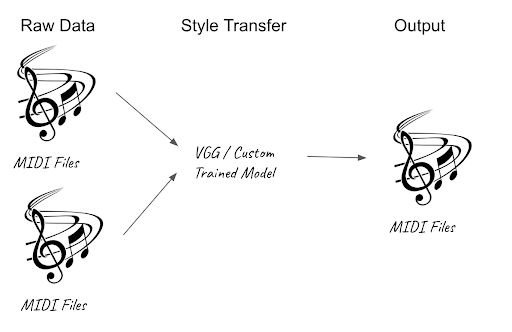
\includegraphics[width=\columnwidth]{normalstruct}}
\centerline{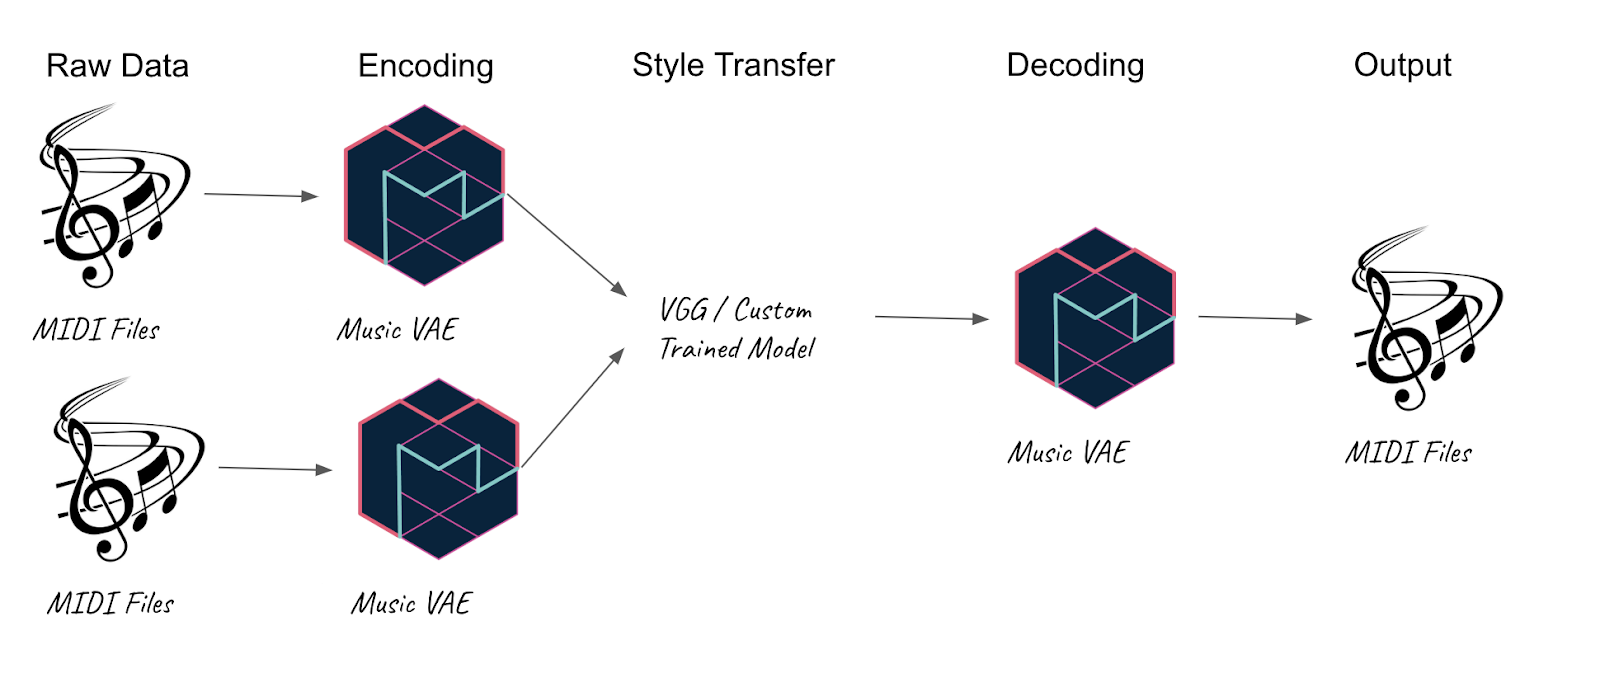
\includegraphics[width=\columnwidth]{vaestruct}}

Figure 1: Diagrams of the music style transfer experiments. Each diagram represents a set of two experiments. Experiment one and two are shown on the left image, while Experiment three and four are shown on the right. 

Experiment 1 - Feed in music files in midi format straight into the VGG model. To be able to do so we copy the music information three times to add an additional dimension to the input tensor. This allows us to mimic the three channeled structure of images. Similar approaches have been used for grayscale image style transfer. 

Experiment 2 - Feed in music files in midi format straight into our Custom Composer Classifier.

Experiment 3 - Encode music files in midi format using our Music VAE, transfer style using the VGG model, and then decode back into midi like format. Note: in this experiment we still expand one of the dimensions to accommodate VGG’s input constraints. 

Experiment 4 - Encode music files in midi format using our Music VAE, transfer style using our Custom Composer Classifier, and then decode back into midi like format.

Whenever we compute the loss using a VGG model for the style transfer we use the Gram-matrix for the style transfer, while when we use the Custom Composer Classifier we use just the dot product

\section{Results}
\label{results}

You can find the full results and our conclusion at our Github: https://github.com/Zhachory1/MusicNST

\centerline{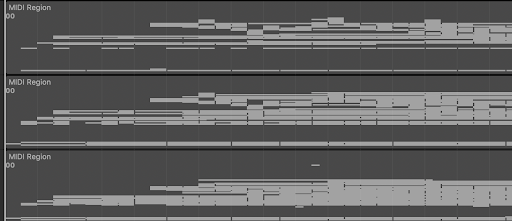
\includegraphics[width=\columnwidth]{tracks}}

These tracks are pulled from iterations 1, 10, and 100 from the Neural Style Transfer model using VGG as the backbone without the VAE preprocessing. You can notice that the model is creating denser formats the more iterations it does. We did not tune the parameter for putting a ratio between content and style loss, which was set at 1:4. Tuning this would've put less emphasis on imposing a style in the content music, which could have proved to be better. 

\centerline{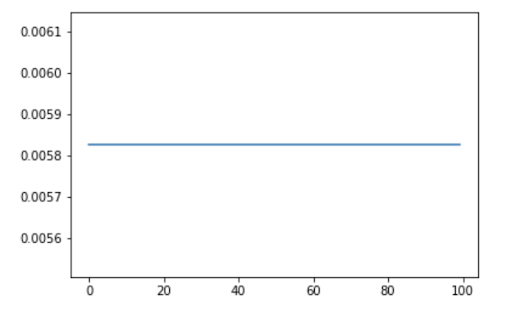
\includegraphics[width=\columnwidth]{flatline}}
\centerline{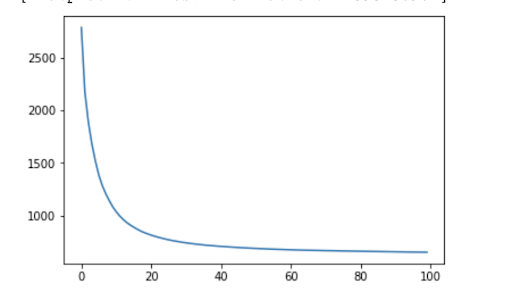
\includegraphics[width=\columnwidth]{curvedline}}

Figure 2: Music neural style transfer loss curvature. The x-axis is number of steps and the y-axis is loss value. The one on the left was generated using our simple music classifier, while the one on the right was generated through a VGG model. 

We believe that our convolutional network was too shallow to transfer music style appropriately. When we trained with deeper networks we were overfitting with more layers. However, when we trained using the VAE and the same network architecture we were underfitting. This hints that we need to explore deeper architectures when dealing with music style transfer. 


Given significant processing constraints we were unable to train a good copy of the music VAE. Therefore, we decided to halt Experiment three and four. We were only able to train our VAE for a few epochs which was insufficient, given that when we tried to use it to retrain a better classifier the results were worse than just feeding in midi files straight in. The accuracy on the test set was about 10\% lower(accuracy on the simple classifier is 50\% and on the one trained with a VAE is 41\%). 

\centerline{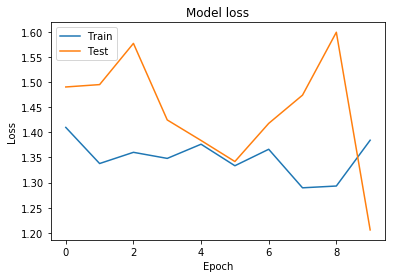
\includegraphics[width=\columnwidth]{badloss}}

Figure 3: Loss curve on test and train on the composer classification model trained using VAE as an encoder over the epochs. 

These results from training the composer classifier with latent code from our VAE were inconclusive since the encoding model was not thoroughly trained. Looking at the distribution of all the Z values, no value went passed 0.0025 and clustered around 0. These low and clustered numbers suggest that we trained with too much emphasis on minimizing the KL divergence. Thus, the reconstruction error was shadowed, consequently taking away our ability to reconstruct our input effectively. 

\section{Conclusion}
\label{conclusion}

Further experiments need to be conducted with a better trained Music VAE. We spent a significant amount of time redesigning the VAE in order to overcome the constraints of the one delivered by the Magenta Team. Unfortunately, it was not effective when used in training because we were unable to fully train it. Moreover, our custom classification model showed good results when trained on test data but was not very robust when used for music style transfer straight from midi files. There were so many nuances from converting midi files, to an intermediate format, to a piano roll/tensor format. There were also many types of channels that could've been pulled from MIDI files, such as onset, offset, active, velocities, along with others. These complications made it difficult to move data around and work with.

\bibliography{MusicNST}
\bibliographystyle{icml2018}

\section{References}

A Roberts, J Engel, C Raffel, C Hawthorne, D Eck, "A hierarchical latent vector model for learning long-term structure in music"- arXiv preprint arXiv:1803.05428, 2018

Brunner, Gino et al. “Symbolic Music Genre Transfer with CycleGAN.” 2018 IEEE 30th International Conference on Tools with Artificial Intelligence (ICTAI) (2018): 786-793.

Gatys, Leon A., et al. “Image Style Transfer Using Convolutional Neural Networks.” 2016 IEEE Conference on Computer Vision and Pattern Recognition (CVPR), 2016, doi:10.1109/cvpr.2016.265.

Higgins, Irina et al. “beta-VAE: Learning Basic Visual Concepts with a Constrained Variational Framework.” ICLR (2017).

Hinton, Geoffrey E. and Ruslan R. Salakhutdinov. “Reducing the dimensionality of data with neural networks.” Science 313 5786 (2006): 504-7 .

Hochreiter, Sepp, and Schmidhuber Jurgen. “Long Short Term Memory.” Long Short Term Memory, Inst. fur Informatik, TUM, 1994.

I. Goodfellow, J. Pouget-Abadie, M. Mirza, B. Xu, D. WardeFarley, S. Ozair, A. Courville, and Y. Bengio, “Generative adversarial nets,” in Advan

Jing, Yongcheng et al. “Neural Style Transfer: A Review.” CoRR abs/1705.04058 (2017): n. pag.

Kingma, Diederik P. and Max Welling. “Auto-Encoding Variational Bayes.” CoRRabs/1312.6114 (2014): n. pag.

Roberts, Adam et al. “A Hierarchical Latent Vector Model for Learning Long-Term Structure in Music.” ICML (2018).

Roberts, Adam. “MusicVAE: Creating a Palette for Musical Scores with Machine Learning.” Magenta, 15 Mar. 2018, magenta.tensorflow.org/music-vae.

Schuster, Mike and Kuldip K. Paliwal. “Bidirectional recurrent neural networks.” IEEE Trans. Signal Processing 45 (1997): 2673-2681.

Sherstinsky, Alex. “Fundamentals of Recurrent Neural Network (RNN) and Long Short-Term Memory (LSTM) Network.” CoRR abs/1808.03314 (2018): n. Pag.

Zhu, Jun-Yan et al. “Unpaired Image-to-Image Translation Using Cycle-Consistent Adversarial Networks.” 2017 IEEE International Conference on Computer Vision (ICCV)(2017): 2242-2251.

\end{document}


% This document was modified from the file originally made available by
% Pat Langley and Andrea Danyluk for ICML-2K. This version was created
% by Iain Murray in 2018, and modified by Alexandre Bouchard in
% 2019. Previous contributors include Dan Roy, Lise Getoor and Tobias
% Scheffer, which was slightly modified from the 2010 version by
% Thorsten Joachims & Johannes Fuernkranz, slightly modified from the
% 2009 version by Kiri Wagstaff and Sam Roweis's 2008 version, which is
% slightly modified from Prasad Tadepalli's 2007 version which is a
% lightly changed version of the previous year's version by Andrew
% Moore, which was in turn edited from those of Kristian Kersting and
% Codrina Lauth. Alex Smola contributed to the algorithmic style files.